\section{Servidor na Nuvem \label{servidorNaNuvem}}

\subsection{Descrição}

O servidor na nuvem é composto por um servidor WebSocket para comunicação entre clientes e casas, um banco de dados em memória para armazenar informações sobre conexões WebSocket ativas, uma API REST para acesso aos dados persistidos, um banco de dados não-relacional para armazenar dados dos sensores, módulos, Morpheus e usuários, um proxy reverso e um \emph{firewall}.

Para fins de prova de conceito, optou-se por prosseguir com uma arquitetura monolítica. A implementação da arquitetura de microsserviços aumentaria consideravelmente a complexidade do projeto, e seus principais benefícios não seriam tão bem aproveitados, visto que o sistema não seria colocado a provas de carga real no momento. Contudo, ressalta-se que o monolito que compõe o servidor na nuvem poderia sim ser implementado como um conjunto de microsserviços, o que seria uma evolução natural à medida que o sistema escala.

\subsection{Características da Implementação}

Com base nos requisitos funcionais e não-funcionais, discutidos na Subseção \ref{sec:requisitos}, foi realizada a implementação na nuvem. Suas características são discutidas em seguida.

\begin{description}

\item \textbf{Comunicação}

\begin{itemize}
\item O servidor permite que Morpheus e aplicativos clientes se comuniquem via WebSocket.
\item Morpheus pode enviar as mensagens provenientes dos módulos físicos, que são: \texttt{configuration}, \texttt{confirmation} e \texttt{data}. Também podem receber mensagens destinadas aos módulos físicos, que são: \texttt{action}, \texttt{configuration} e \texttt{data}.
\item Morpheus pode receber mensagens de registro e remoção de módulo para definir quais dispositivos ele gerencia.
\item Morpheus pode enviar mensagens de \texttt{report}.
\item Os aplicativos cliente podem enviar as mensagens correspondentes a interações do usuário, que são: \texttt{action} e \texttt{configuration}. Também podem receber mensagens provenientes dos módulos físicos, que são: \texttt{confirmation} e \texttt{data}.
\item Aplicativos cliente podem receber mensagens de \texttt{report}.
\item Aplicativos cliente podem receber o status de conectividade dos Morpheus e receber notificações quando um Morpheus for desconectado.
\end{itemize}

\item \textbf{Persistência de Dados}

\begin{itemize}
\item O servidor persiste dados de usuário, de configurações de Morpheus e módulo e de mensagens de dados (\texttt{data} e \texttt{report}).
\end{itemize}

\item \textbf{Gerenciamento de Dados}

\begin{itemize}
\item O servidor oferece uma API REST para leitura e escrita de dados de usuário, configurações de Morpheus e de módulos.
\end{itemize}

\item \textbf{Conexões}

\begin{itemize}
\item O servidor permite o estabelecimento de conexões HTTPS seguras e criptografadas.
\item O \emph{firewall} bloqueia conexões em portas que não estão sendo utilizadas.
\end{itemize}

\end{description}

\subsection{Tecnologias Utilizadas}

O servidor foi desenvolvido usando Node.js\footnote{https://nodejs.org}, um ambiente em tempo de execução para código em JavaScript. Sua arquitetura usa um modelo orientado a eventos e realiza a execução de comandos concorrentemente sem bloquear o servidor. Assim, servidores em Node.js conseguem alcançar uma melhor escalabilidade, suportando múltiplas conexões simultâneas sem impactos de performance.

Para a persistência de dados, foi escolhido o MongoDB\footnote{https://www.mongodb.com/}, banco de dados não-relacional baseado em documentos. A facilidade de integração com JavaScript e Node.js, a similaridade dos documentos com objetos JSON e a natureza dos dados de sensores foram as motivações para sua escolha como banco de dados principal.

Contudo, não são apenas informações sobre usuários e dispositivos e dados coletados pelos sensores que precisam ser armazenados. Para gerenciar quais Morpheus estão conectados à nuvem e a quais aplicativos suas informações em tempo real devem ser enviadas, é usado o Redis\footnote{https://redis.io/}, banco de dados em memória. Redis é popularmente usado para fins como cache, mensageria e implementação de filas. No caso do Hedwig, ele é utilizado para armazenar informações de sessão, que são temporárias e requerem baixas latências para leitura e escrita.

Para implementar a comunicação entre aplicativos e casas, foi escolhida a biblioteca Socket.io\footnote{https://socket.io/}, que fornece uma API de alto nível para troca de informações bidirecional por meio de eventos. Além de abstrair a API de baixo nível do protocolo de WebSockets, o Socket.io já fornece eventos referentes ao status da conexão, facilitando o disparo de notificações caso o controlador de uma casa seja desconectado, e implementa um \emph{fallback} para clientes que não suportam o protocolo de WebSocket. Por exemplo, se um usuário acessa um aplicativo por meio de um navegador antigo, a troca de dados continua sendo feita por meio de \emph{long polling}.

A arquitetura possui um proxy reverso que é responsável por enviar as requisições ao servidor em Node.js. Para isso, foi usado o nginx\footnote{https://nginx.org/}, popularmente utilizado como servidor HTTP e proxy genérico para TCP e UDP. Ele permite a configuração de conexões seguras via HTTPS e dispensa a necessidade de delegar privilégios para acessar as portas reservadas 80 e 443 ao processo que roda o servidor Node.js.

Por fim, foi usada a ferramenta padrão do Ubuntu para \emph{firewall}, ufw, que permite criar regras para bloquear tráfego IPv4 e IPv6.

As tecnologias apresentadas aqui favorecem a escalabilidade do sistema. O Node.js possui um modo de execução \emph{cluster}, no qual processos filhos ou \emph{workers} são criados a partir de um processo pai ou \emph{master} por meio de \emph{forking}, sendo possível assim aproveitar todas as CPUs de uma máquina \cite{nodejscluster}. O MongoDB suporta técnicas de \emph{sharding}, que é um método para distribuir dados em múltiplas máquinas para armazenar grandes quantidades de dados e garantir alta vazão de leituras e escritas \cite{mongodbsharding}. O Redis também pode ser escalado por meio de ``clusterização''. Já o nginx possui uma arquitetura que consegue lidar com centenas de milhares de requisições sem bloquear sua máquina de estados, otimizando o número de processos para diminuir o tempo gasto em mudanças de contexto \cite{nginxscalability}.

\begin{figure}[H]
	\centering
	\caption{Componentes e implementação na nuvem}
  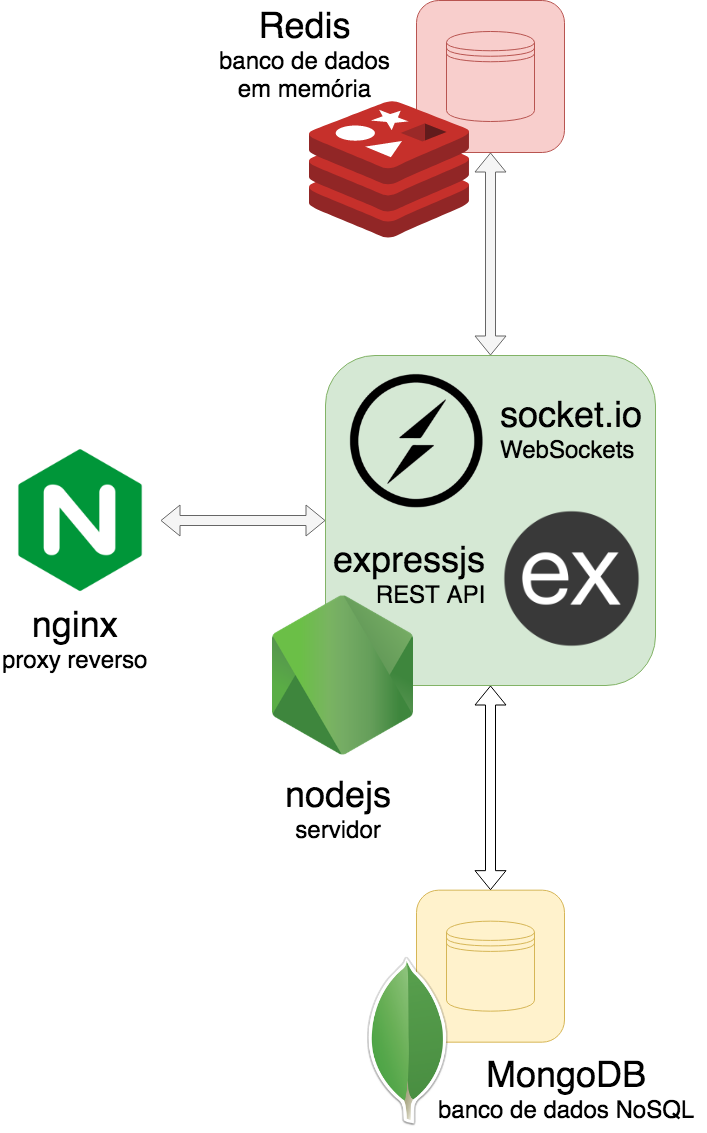
\includegraphics[width=0.5\textwidth]{componentesNuvem}
\label{fig:componentesNuvem}
\end{figure}

\subsection{Tratamento de Eventos}

O servidor na nuvem possui uma arquitetura baseada em eventos, que transmitem dados, ações, configurações e confirmações e podem ser provenientes dos Morpheus ou dos aplicativos clientes conectados. O servidor também pode emitir seus próprios eventos para tais entidades conectadas ouvirem. Nessa seção, as rotinas de tratamento para cada tipo de evento são sucintamente descritas.

\paragraph{Conexão (\texttt{connection})}
\begin{itemize}
\item \textbf{Descrição}: um novo dispositivo se conecta à nuvem.
\item \textbf{Emitido por}: Morpheus, aplicativos clientes.
\item \textbf{Tratamento}: é criada uma \emph{string} única de identificação para a nova conexão.
\end{itemize}

\paragraph{Identificação de Dispositivo Conectado (\texttt{hello})}
\begin{itemize}
\item \textbf{Descrição}: ao se conectar à nuvem, um novo dispositivo se identifica como Morpheus ou aplicativo cliente. Em ambos os casos, é enviado também a identificação serial do Morpheus --- no caso dos aplicativos, seria o Morpheus do qual se deseja receber notificações em tempo real. Caso um aplicativo queira receber notificações de múltiplos Morpheus, devem ser enviados múltiplos eventos de \texttt{hello}.
\item \textbf{Emitido por}: Morpheus, aplicativos clientes.
\item \textbf{Tratamento}: o identificadores de conexão, os tipos de dispositivos e os identificadores seriais do Morpheus são salvos no Redis. Assim, é possível buscar qual é a conexão correspondente a cada dispositivo conectado.
Além disso, se já existem dados salvos no Redis a respeito de aplicativos ou Morpheus que referenciam ao mesmo serial de Morpheus, são enviados a eles eventos de \texttt{hello}. Um caso de uso para tal funcionalidade é a possibilidade de aplicativos saberem se todos os controladores locais de uma residência estão online.
\end{itemize}

\paragraph{Ação (\texttt{action})}
\begin{itemize}
\item \textbf{Descrição}: é enviada uma requisição de ação a um módulo.
\item \textbf{Emitido por}: aplicativos clientes.
\item \textbf{Tratamento}: é verificado se o Morpheus responsável por repassar essa requisição ao módulo físico está conectado. Se sim, o evento de \texttt{action} é re-emitido somente a ele.
\end{itemize}

\paragraph{Configuração (\texttt{configuration})}
\begin{itemize}
\item \textbf{Descrição}: é enviada uma requisição de configuração a um módulo.
\item \textbf{Emitido por}: aplicativos clientes.
\item \textbf{Tratamento}: é verificado se o Morpheus responsável por repassar essa requisição ao módulo físico está conectado. Se sim, o evento de \texttt{configuration} é re-emitido somente a ele.
\end{itemize}

\paragraph{Confirmação (\texttt{confirmation})}
\begin{itemize}
\item \textbf{Descrição}: é enviada uma confirmação de ação ou configuração a um aplicativo.
\item \textbf{Emitido por}: Morpheus.
\item \textbf{Tratamento}: é verificado se existem aplicativos correspondentes a esse Morpheus conectados à nuvem. Se sim, o evento de \texttt{confirmation} é re-emitido a todos eles. Isso é uma simplificação que obriga os aplicativos a tratarem o recebimento desse tipo de evento por si mesmos.
\end{itemize}

\paragraph{Dados (\texttt{data})}
\begin{itemize}
\item \textbf{Descrição}: é enviada uma atualização do estado do módulo físico e seus sensores.
\item \textbf{Emitido por}: Morpheus.
\item \textbf{Tratamento}: é verificado se existem aplicativos correspondentes a esse Morpheus conectados à nuvem. Se sim, o evento de \texttt{data} é re-emitido a todos eles. Além disso, esses dados são persistidos no MongoDB.
\end{itemize}

\paragraph{Relatório (\texttt{report})}
\begin{itemize}
\item \textbf{Descrição}: é enviada um relatório de configurações do Morpheus.
\item \textbf{Emitido por}: Morpheus.
\item \textbf{Tratamento}: é verificado se existem aplicativos correspondentes a esse Morpheus conectados à nuvem. Se sim, o evento de \texttt{report} é re-emitido a todos eles. Além disso, esses dados são persistidos no MongoDB.
\end{itemize}

\paragraph{Desconexão (\texttt{disconnect})}
\begin{itemize}
\item \textbf{Descrição}: um dispositivo se desconecta da nuvem.
\item \textbf{Emitido por}: Morpheus, aplicativos clientes.
\item \textbf{Tratamento}: as entradas no Redis relacionada a essa conexão são deletadas. Se o dispositivo que se desconectou foi um Morpheus, é emitido um evento de \texttt{bye} a todos os aplicativos conectados que estavam ouvindo atualizações desse Morpheus. Dessa forma, podem ser implementadas mensagens de erro e avisos ao usuário.
\end{itemize}

\subsection{Infraestrutura}

Para hospedar o servidor do Hedwig, foi utilizado o serviço de computação na nuvem Digital Ocean \footnote{https://www.digitalocean.com/}. Com ele, foi possível implantar o servidor em uma instância que roda Ubuntu 16.04.3 x64, com única CPU, 512MB de memória, 20GB de armazenamento de disco SSD e 1000GB de cota disponível para transferência de dados. O data center que hospeda essa instância fica em Nova Iorque.

\subsection{Segurança}

O servidor na nuvem suporta conexões HTTPS, permitindo que navegadores verifiquem a autenticidade do servidor e garantindo a privacidade e integridade dos dados transmitidos. Para isso, foi usado o Let's Encrypt\footnote{https://letsencrypt.org}, uma autoridade de certificação aberta, gratuita e automatizada. O Let's Encrypt usa o protocolo ACME (\emph{Automatic Certificate Management Environment}) para automatizar a comunicação entre autoridade e candidato para assegurar a autenticidade deste e conceder-lhe certificados de forma rápida e prática. É realizado um teste para verificar que o candidato possui controle sobre o domínio e, então, é gerado um certificado válido por 90 dias que pode ser renovado a qualquer momento. Para usá-lo no servidor, basta acrescentar novas configurações ao nginx.

Além disso, outra medida de segurança foi usar o \emph{firewall} ufw para bloquear conexões nas portas TCP que não estão sendo usadas.

\subsection{Operação}

O serviço Keymetrics\footnote{https://keymetrics.io/} permite verificar se o servidor na nuvem está online, monitorar o uso de CPU e de memória, investigar a ocorrência de erros e realizar ações comuns, como reiniciar o processo do servidor, por meio de uma interface amigável. Investir em um sistema de monitoramento como esse auxilia tanto a manutenção preventiva como a corretiva, o que é essencial para um sistema de casa inteligente que tem a disponibilidade como requisito prioritário.

\begin{figure}[H]
	\centering
	\caption{Monitoramento do servidor na nuvem}
  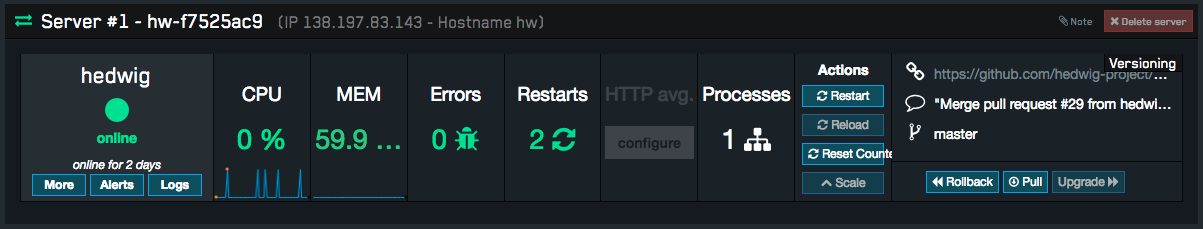
\includegraphics[width=1.0\textwidth]{keymetrics}
\label{fig:keymetrics}
\end{figure}

Outro ponto abordado é o uso de logs, arquivos que gravam eventos relevantes que acontecem no sistema. Eles podem ser usados para realizar a auditoria de falhas ocorridas e compreender melhor o funcionamento de um programa. Por questões de simplicidade, para classificar os eventos, o servidor na nuvem do Hedwig usa três dos sete níveis de severidade definidos pelo padrão syslog \cite{rfc5424}: \emph{error}, \emph{warning} e \emph{informational}. O servidor implementa um esquema de rotação de logs, criando arquivos individuais para cada dia, o que facilita o arquivamento de logs muito antigos e a pesquisa de eventos específicos. Com esse sistema, também é possível filtrar eventos de severidades diferentes em arquivos separados.
